\documentclass[journal,12pt,twocolumn]{IEEEtran}

\usepackage{setspace}
\usepackage{gensymb}
\singlespacing
\usepackage[cmex10]{amsmath}

\usepackage{amsthm}

\usepackage{mathrsfs}
\usepackage{txfonts}
\usepackage{stfloats}
\usepackage{bm}
\usepackage{cite}
\usepackage{cases}
\usepackage{subfig}

\usepackage{longtable}
\usepackage{multirow}

\usepackage{enumitem}
\usepackage{mathtools}
\usepackage{steinmetz}
\usepackage{tikz}
\usepackage{circuitikz}
\usepackage{verbatim}
\usepackage{tfrupee}
\usepackage[breaklinks=true]{hyperref}
\usepackage{graphicx}
\usepackage{tkz-euclide}

\usetikzlibrary{calc,math}
\usepackage{listings}
    \usepackage{color}                                            %%
    \usepackage{array}                                            %%
    \usepackage{longtable}                                        %%
    \usepackage{calc}                                             %%
    \usepackage{multirow}                                         %%
    \usepackage{hhline}                                           %%
    \usepackage{ifthen}                                           %%
    \usepackage{lscape}     
\usepackage{multicol}
\usepackage{chngcntr}

\DeclareMathOperator*{\Res}{Res}

\renewcommand\thesection{\arabic{section}}
\renewcommand\thesubsection{\thesection.\arabic{subsection}}
\renewcommand\thesubsubsection{\thesubsection.\arabic{subsubsection}}

\renewcommand\thesectiondis{\arabic{section}}
\renewcommand\thesubsectiondis{\thesectiondis.\arabic{subsection}}
\renewcommand\thesubsubsectiondis{\thesubsectiondis.\arabic{subsubsection}}


\hyphenation{op-tical net-works semi-conduc-tor}
\def\inputGnumericTable{}                                 %%

\lstset{
%language=C,
frame=single, 
breaklines=true,
columns=fullflexible
}
\begin{document}

\newcommand{\BEQA}{\begin{eqnarray}}
\newcommand{\EEQA}{\end{eqnarray}}
\newcommand{\define}{\stackrel{\triangle}{=}}
\bibliographystyle{IEEEtran}
\raggedbottom
\setlength{\parindent}{0pt}
\providecommand{\mbf}{\mathbf}
\providecommand{\pr}[1]{\ensuremath{\Pr\left(#1\right)}}
\providecommand{\qfunc}[1]{\ensuremath{Q\left(#1\right)}}
\providecommand{\sbrak}[1]{\ensuremath{{}\left[#1\right]}}
\providecommand{\lsbrak}[1]{\ensuremath{{}\left[#1\right.}}
\providecommand{\rsbrak}[1]{\ensuremath{{}\left.#1\right]}}
\providecommand{\brak}[1]{\ensuremath{\left(#1\right)}}
\providecommand{\lbrak}[1]{\ensuremath{\left(#1\right.}}
\providecommand{\rbrak}[1]{\ensuremath{\left.#1\right)}}
\providecommand{\cbrak}[1]{\ensuremath{\left\{#1\right\}}}
\providecommand{\lcbrak}[1]{\ensuremath{\left\{#1\right.}}
\providecommand{\rcbrak}[1]{\ensuremath{\left.#1\right\}}}
\theoremstyle{remark}
\newtheorem{rem}{Remark}
\newcommand{\sgn}{\mathop{\mathrm{sgn}}}
\providecommand{\abs}[1]{\vert#1\vert}
\providecommand{\res}[1]{\Res\displaylimits_{#1}} 
\providecommand{\norm}[1]{\lVert#1\rVert}
%\providecommand{\norm}[1]{\lVert#1\rVert}
\providecommand{\mtx}[1]{\mathbf{#1}}
\providecommand{\mean}[1]{E[ #1 ]}
\providecommand{\fourier}{\overset{\mathcal{F}}{ \rightleftharpoons}}
%\providecommand{\hilbert}{\overset{\mathcal{H}}{ \rightleftharpoons}}
\providecommand{\system}{\overset{\mathcal{H}}{ \longleftrightarrow}}
	%\newcommand{\solution}[2]{\textbf{Solution:}{#1}}
\newcommand{\solution}{\noindent \textbf{Solution: }}
\newcommand{\cosec}{\,\text{cosec}\,}
\providecommand{\dec}[2]{\ensuremath{\overset{#1}{\underset{#2}{\gtrless}}}}
\newcommand{\myvec}[1]{\ensuremath{\begin{pmatrix}#1\end{pmatrix}}}
\newcommand{\mydet}[1]{\ensuremath{\begin{vmatrix}#1\end{vmatrix}}}
\numberwithin{equation}{subsection}
\makeatletter
\@addtoreset{figure}{problem}
\makeatother
\let\StandardTheFigure\thefigure
\let\vec\mathbf
\renewcommand{\thefigure}{\theproblem}
\def\putbox#1#2#3{\makebox[0in][l]{\makebox[#1][l]{}\raisebox{\baselineskip}[0in][0in]{\raisebox{#2}[0in][0in]{#3}}}}
     \def\rightbox#1{\makebox[0in][r]{#1}}
     \def\centbox#1{\makebox[0in]{#1}}
     \def\topbox#1{\raisebox{-\baselineskip}[0in][0in]{#1}}
     \def\midbox#1{\raisebox{-0.5\baselineskip}[0in][0in]{#1}}
\vspace{3cm}
\title{Assignment 1}%number
\author{B. Ramana}
\maketitle
\newpage
\bigskip
\renewcommand{\thefigure}{\theenumi}
\renewcommand{\thetable}{\theenumi}
\newcommand*{\permcomb}[4][0mu]{{{}^{#3}\mkern#1#2_{#4}}}
\newcommand*{\perm}[1][-3mu]{\permcomb[#1]{P}}
\newcommand*{\comb}[1][-1mu]{\permcomb[#1]{C}}
Download all python codes from 
\begin{lstlisting}
https://github.com/B.Ramana/Matrix-theory/codes
\end{lstlisting}
%
and latex-tikz codes from 
%
\begin{lstlisting}
https://github.com/B.Ramana/Matrix-theory
\end{lstlisting}
\section*{Question No. 2.20}
construct $\triangle ABC$ given that $\angle A=60\degree,\angle B=30\degree$ and $AB$=5.8
\section*{Solution}
Given,
\begin{align}
\angle A=60\degree,\angle B=30\degree AB=5.8
\end{align}
let's first drawn a diagram.
To construct $\triangle ABC$,we first need to find $\angle C$
Finding $\angle C$ in$\triangle ABC$
\begin{align}
\angle A+\angle B+\angle C=180\degree\\
60\degree+30\degree+\angle C = 180\degree\\
90\degree+\angle C=180\degree\\
\angle C=180\degree-90\degree\\
\angle C=90\degree    
\end{align}
Now finding "Opposite" and "adjacent" where "hypotenuse"is given $AB$=58.

Case:1
\begin{align}
\angle B&=30\degree
\\
\text{hypotenuse}&=5.8
\\
\text{Opposite side}&=\frac {\text{hypotenuse}}{\sin30\degree}
\\
\text{Opposite side} &=\frac {5.8}{0.5}
\\
\text{Opposite side}&=2.9;
 \\
\text{Adjacent side}&=\frac {\text{hypotenuse}}{\cos30\degree}
 \\
\text{Adjacent side} &=\frac {5.8}{0.866}\\
\text{Adjacent side}&=4.10;
\end{align} 
Case:2
\begin {align}
let\angle A& =60\degree
\\
\text{hypotenus}&=5.8
\\
\text{Opposite side}&=\frac{\text{hypotenuse}}{sin60\degree}
\\
\text{Opposite side}&=\frac{5.8}{0.866}
\\
\text{Opposite side}&=4.10;
\\
\text {Adjacent side}&=\frac{\text{hypotenuse}}{cos60\degree}
\\
\text{Adjacent side }&=\frac{5.8}{0.5}
\\
\text{Adjacent side}&=2.9;
\\
\end{align}
By solving ,we get Values :
\begin{align}
\implies a&=4.10;
\\
\implies b&=2.9;
\\
\implies c&=5.8
\\
\end{align}
The  Vertices of $\triangle ABC$ are
\begin{align}
 \Vec {A}&=\myvec{0\\ c}=\myvec{0\\5.8} \\ \Vec{B}&=\myvec{a\\ 0} =\myvec{4.10\\ 0}\\ \Vec{C}&=\myvec {0\\ 0}
\end{align}
Plot the $\triangle ABC$ is as follows:
\begin{figure}[h!]
\centering
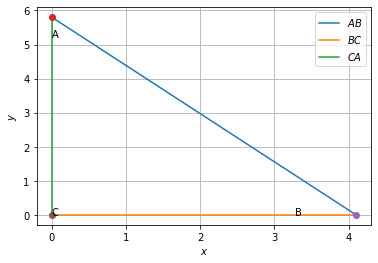
\includegraphics[width=\columnwidth]{Figure 1.png}
\caption{$\triangle ABC$}
\label{triangle ABC}
\end{figure}
\end{document}